% Change the title, course, author, and professor details
\SheetTitle{Problem Set Title}{Course Name}{Author Name}

\section{Section Title}

% Example of a problem
\vspace{0.9cm}
\begin{p}
  Problem statement here.
\end{p}

\begin{solution}
  Solution goes here. Use the \emph{italic} or \textbf{bold} text as needed.
  
  You can add figures (Fig.~\ref{fig:example}) with captions and labels:
  \begin{figure}[H]
    \centering
    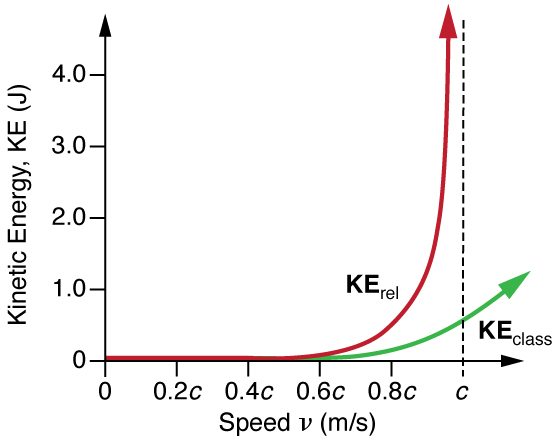
\includegraphics[width=0.5\textwidth]{figures/example.jpg}
    \caption{\emph{Caption for the example figure.}}
    \label{fig:example}
  \end{figure}

  Continue with the rest of the solution. For equations, you can use:
  \begin{equation}
    E = mc^2
  \end{equation}

  or 

  \begin{align*}
    E &= mc^2 \\
    F &= ma
  \end{align*}

  
  Add more text here, or conclude your solution.

\end{solution}

\begin{remark}
  Remarks can be added at the beginning, end, or in the solution.
\end{remark}

\vspace{\lineskip}

\begin{proof}
  Proofs can be added at the beginning, end, or in the solution.
\end{proof}

% You can copy the above block for multiple problems and solutions.

\footnotetext{Collaborators or other acknowledgments can be added here.}
